\chapter{Discrete Representations and Generative Modeling}

\section{Introdcution}
The \textbf{Discretization} is the process of dividing continuos phenomena into \textbf{distinct parts}, resonates deeply with how humans understand and interact with the world.

It is not just a computational tool but a reflection of a fundamental cognitive process. It has been explored in philosopy, science, and mathematics for centuries.

\subsection{Immanuel Kant}
Philosophers have long pondered how humans make sense of the
continuous and often chaotic flow of reality.
\begin{wrapfigure}{r}{0.2\textwidth}
    \centering
    \vspace{-10pt}
    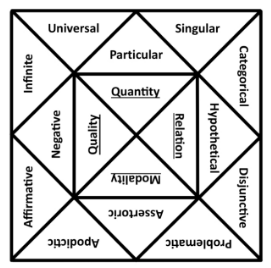
\includegraphics[width=\linewidth]{images/Kant.png}
    \label{fig:Scaled Dot Product Attention}
    \vspace{-10pt}
\end{wrapfigure}
\textbf{Immanuel Kant}, in his seminal Critique of Pure Reason (1781), argued
that the human mind does not passively receive sensory input but actively
structures it.

According to Kant, this structuring process involves applying innate \textbf{categories of understanding} to the manifold of experience – a form of \textbf{conceptual discretization}, to borrow a modern term, that transforms raw sensory data into coherent and intelligible knowledge.

\subsection{René Descartes}
Similarly, René Descartes revolutionized mathematics and philosophy by introducing the Cartesian coordinate system in his 1637 work La Géométrie.
\begin{wrapfigure}{r}{0.2\textwidth}
    \centering
    \vspace{-10pt}
    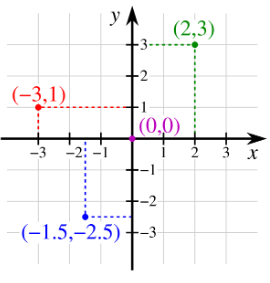
\includegraphics[width=\linewidth]{images/renè.png}
    \label{fig:Scaled Dot Product Attention}
    \vspace{-10pt}
\end{wrapfigure}
By discretizing continuous space into measurable dimensions of x and y, Descartes laid the groundwork for modern analytical geometry.

This act of partitioning space into discrete points not only enabled scientific progress but also reflected a deeper philosophical position: that understanding the infinite requires reducing itto finite, manageable parts.

\subsection{Why Discrete Representations?}
Many real-world domains are inherently \textbf{discrete}, and modeling them with continuous representation may miss important structural properties. For example like:
\begin{compactitemize}
    \item \textbf{Language} consist of sequence of discete symbols (word, subword).
    \item \textbf{Images} are stored as discrete grids of pixels with quantized color values.
    \item \textbf{Music and speech} are often represented symbolically (e.g, notes, phonemes).
\end{compactitemize}


In the context of artificial learning systems, dicrete models and representation/enable:
\begin{compactitemize}
    \item \textbf{Efficient Compression}
    Discrete latent variables are significantly \textbf{easier to encode compactly}. This facilitates better data compression and representation efficiency, as the information is stored using distinct, finite codes.
    
    \item \textbf{Symbolic Reasoning}
    Discrete representations enable the direct application of \textbf{formal logic} and \textbf{symbolic manipulation}. This is crucial for tasks requiring transparent, step-by-step reasoning, such as applying mathematical or logical rules.

    \item \textbf{Modular Design}
    Discrete mechanisms facilitate the creation of \textbf{modular and specialized architectures}. In systems like the \textbf{Mixture of Experts (MoE)}, a discrete gating function selects specific experts for computation, leading to:
\end{compactitemize}
\begin{figure}[H]
    \centering
    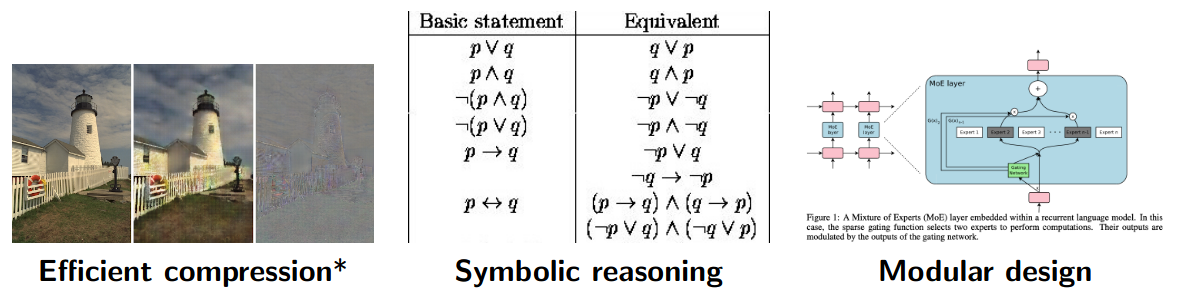
\includegraphics[width=0.9\textwidth]{images/D1.png}
    \label{fig:MHA2}
\end{figure}

\subsection{Problem with descritization}
So if we say since the beginning of the course, each NN is trained through gradient descent, this implies that each function that we use is differentiable.

But many times when we do discretization, we use functions like argmax or argmin that clearly are not differentiable functions. To give an example, if we try to run the code showed below, it won't run because we cannot compute the gradient of the argmax function.
\begin{figure}[H]
    \centering
    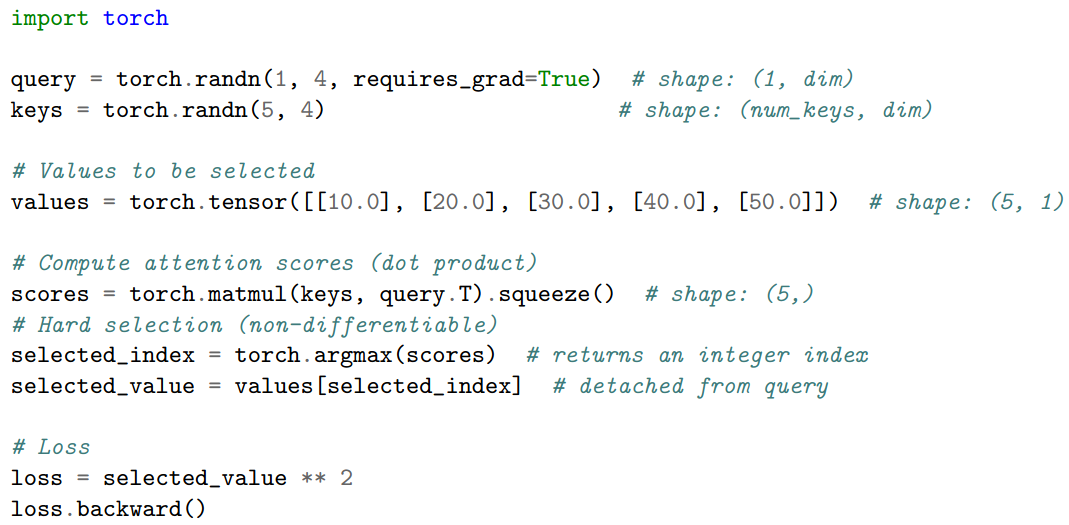
\includegraphics[width=0.9\textwidth]{images/code.png}
    \label{fig:MHA2}
\end{figure}

A possible solutions for this problem are:
\begin{compactitemize}
    \item \textbf{VQ-VAEs} involve straight-through estimators
    \item \textbf{Pixel-RNN} employ autoregressive training
    \item Surrogate gradients (e.g., Gumbel Softmax)
\end{compactitemize}

\section{Vector Quantized-Variational Autoencoders}
While Variational Autoencoders (VAEs) are effective at learning a compressed, lower-dimensional representation of the training data and providing an explicit density estimation for generating new samples, they suffer from two major problems.

The most noticeable issue is their tendency to generate \textbf{blurry}, unrealistic outputs. This is because VAEs typically use a pixel-wise reconstruction loss (like Mean Squared Error), which penalizes variance and tends to favor an average of possible outputs rather than sharp, high-frequency details. This averaging effect results in blurry images.
\begin{figure}[H]
    \centering
    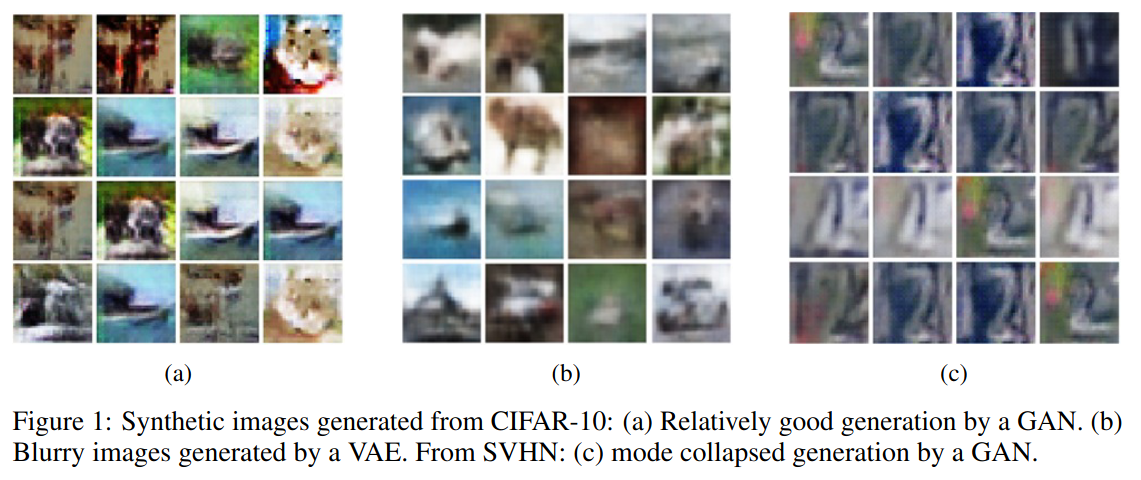
\includegraphics[width=0.8\textwidth]{images/D2.png}
    \label{fig:MHA2}
\end{figure}
The second core issue is \textbf{Posterior Collapse}. This occurs when the encoder's variational posterior distribution collapses quickly to the prior distribution (often a simple Gaussian) early in the training process. When this happens, the latent variables (z) essentially stop carrying any meaningful information about the input image (x), effectively making the generative process redundant. Consequently, the decoder learns to ignore the latent code and generates images based solely on the overall structure of the training dataset. This collapse is often difficult to reverse; once the encoder has settled on the uninformative prior, it rarely recovers without specific interventions or architectural changes.

The are two possbile solutions:
\begin{compactitemize}
    \item \textbf{$\beta-VAE$} it simply introduces a hyperparameters $\beta$ to weigh the importance of the KL divergence within the ELBO objective:
    \[
        \mathcal{L}_{\text{VAE}} = \mathbb{E}_{z \sim Q(z|X)}[\log P(X|z)] - \beta D_{KL}[Q(z|X)\|P(z)]
    \]
    \item \textbf{Vector Quantized-Variational Autoencode}
\end{compactitemize}

\subsection{Vector Quantized-Variational Autoencode (VQ-VAE)}
VQ-VAE is the first model to use \textbf{discrete latent variables} successfully, it uses the whole latent space and avoids the posterior collapse problem.

VQ-VAE is a \textbf{standard} autoencoder network, with an ancoder and a decoder network. Differently from VAEs, the latent embedding space does \textbf{not follow a Gaussian distribution}.

The model takes an input $x$, that is passed through an encoder network, the encoder produces a \textbf{continuos} output $z_e(x)$.
\begin{wrapfigure}{r}{0.5\textwidth}
    \centering
    \vspace{-10pt}
    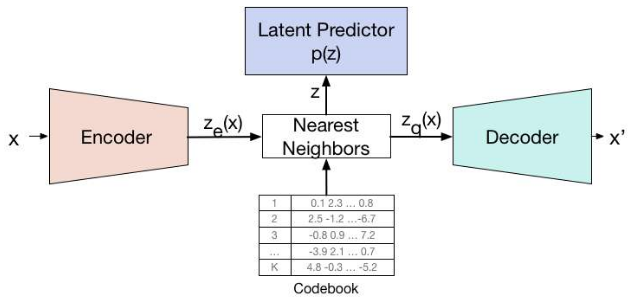
\includegraphics[width=\linewidth]{images/VQ1.png}
    \label{fig:Scaled Dot Product Attention}
    \vspace{-10pt}
\end{wrapfigure}
The latent space is defined through a \textbf{learnable} lookup table, also called \textbf{codebook}, $e \in R^{KxD}$.

$K$ is the size of the discrete latent space and $D$ is the dimensionality of each latent embedding vector. Hence, the codebook is $KxD$.

Each of the $K$ embedding vectors $e_i \in R^D, i=1,2, ... , K$ is learnable through gradient descent.

Given $z_e(x)$, the discrete latent variable $z$ is computed by a \textbf{nearest neighbour look-up} using the shared embedding space.
$$q(z = k|x) =
\begin{cases}
1 & \text{se } k = \underset{j}{\operatorname{argmin}} \|z_e(x) - e_j \|_2^2 \\
0 & \text{altrimenti}
\end{cases}$$
The proposal distribution $q(z=k|x)$ is \textbf{deterministic}.

The input to the decoder is the corresponding embedding vector $e_k$.
$$z_q(x) = e_k, \quad \text{where } k = \underset{j}{\operatorname{argmin}} \|z_e(x) - e_j \|_2^2$$

The complete set of parameters are union of parameters of the encoder, decoder, and the embedding space $e$.
\begin{figure}[H]
    \centering
    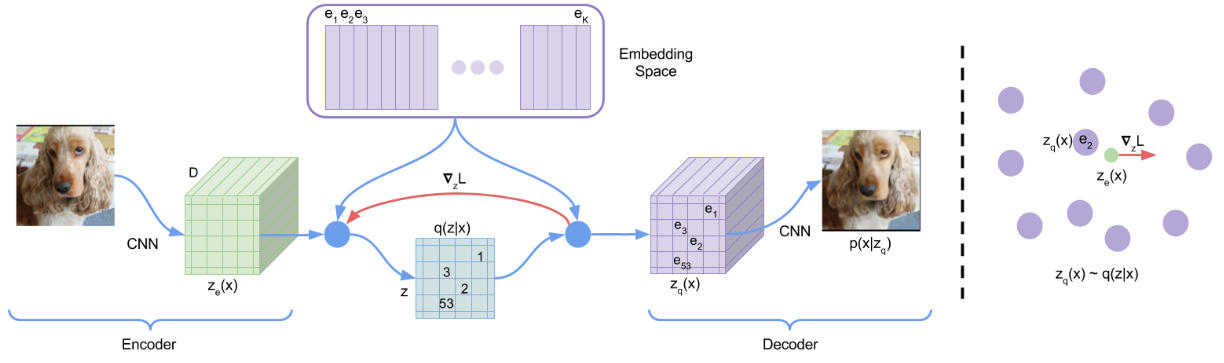
\includegraphics[width=1\textwidth]{images/VQ2.png}
    \caption{VQ-VAE: overall architecture}
    \label{fig:MHA2}
\end{figure}

\subsection{VQ-VAE: Learning}

One can interpret the forward computation pipeline of a VQ-VAE as a standard autoencoder equipped with a peculiar non-linearity that maps the continuous latent vectors into a \textbf{1-of-K} discrete embedding.  
However, this discretization step introduces a major difficulty:  
\textbf{the quantization operation (nearest neighbour lookup) is non-differentiable}.  

Discrete operators such as \texttt{argmax}, \texttt{round} and \texttt{quantize} break the gradient flow during backpropagation.  
To address this issue, VQ-VAE employs a simple but extremely effective technique: the \textbf{Straight-Through Gradient Estimator (STE)}.

\subsubsection{Straight-Through Gradient Estimation}

The key idea behind the STE is to use the discrete code in the forward pass while pretending that the quantization function is the identity during the backward pass.

\begin{itemize}
    \item \textbf{Forward pass:}  
    \[
        z_q = \text{quantize}(z_e)
    \]
    typically via nearest neighbour search in the codebook.
    
    \item \textbf{Backward pass (approximate):}  
    \[
        \frac{\partial L}{\partial z_e} \approx \frac{\partial L}{\partial z_q}
    \]
    The quantization is ignored during backpropagation and treated as the identity function.
\end{itemize}

This trick is widely used beyond VQ-VAEs, for example in:
\begin{compactitemize}
    \item \textbf{Binary neural gates}: forward as a step , backward as a  sigmoid;
    \item \textbf{Neural architecture search} and routing;
    \item \textbf{Pruning and gating mechanisms}.
\end{compactitemize}

\subsection{VQ-VAE: Training Objective}

A critical point is that, due to the straight-through estimator, the embedding vectors $e_i$ in the codebook receive \textbf{no gradient} from the reconstruction loss $\log p(x|z_q(x))$.  
Thus, an additional mechanism is needed to update the codebook.  

VQ-VAE adopts a classical strategy from dictionary learning: \textbf{Vector Quantization}, implemented via simple mean squared error (MSE) terms.

\[
    \mathcal{L} =
    \underbrace{\log p(x|z_q(x))}_{\text{Reconstruction error}}
    +
    \underbrace{\| \text{stopgrad}[z_e(x)] - z_q(x) \|_2^2}_{\text{VQ term}}
    +
    \beta \underbrace{\| z_e(x) - \text{stopgrad}[z_q(x)] \|_2^2}_{\text{Commitment term}}
\]

\paragraph{Interpretation of the three loss components}
\begin{compactitemize}
    \item \textbf{Reconstruction error}  
    Trains only the decoder, encouraging it to reconstruct the input from the selected codeword.

    \item \textbf{Vector Quantization term}  
    Updates the codebook embeddings.  
    It moves each embedding vector $e_k$ closer to the encoder outputs that selected it.

    \item \textbf{Commitment term}  
    Trains the encoder to produce latent vectors $z_e(x)$ that remain close to the chosen codeword.  
    This prevents the encoder from excessively roaming in latent space and promotes stability.
\end{compactitemize}

\paragraph{The stop-gradient operator}
The operator \texttt{stopgrad[$\cdot$]} treats its argument as a constant during backpropagation.  
This allows separating which parts of the loss update the encoder and which parts update the codebook.

\begin{compactitemize}
    \item The \textbf{decoder} optimizes only the reconstruction term.
    \item The \textbf{encoder} optimizes the reconstruction + commitment terms.
    \item The \textbf{embedding space} (codebook) is optimized by the VQ term only.
\end{compactitemize}

This separation is crucial to maintain stable training and prevent collapse of the discrete representations.

\begin{algorithm}[H]
    \caption{VQ-VAE Training Step}
    \textbf{Require:} input $x$, encoder $E(\cdot)$, decoder $D(\cdot)$, codebook $\{e_k\}_{k=1}^K$
    
    $z_e \leftarrow E(x)$ \tcp*[r]{encode input}
    $k \leftarrow \arg\min_j \| z_e - e_j \|_2^2$ \tcp*[r]{nearest codebook entry}
    $z_q \leftarrow e_k$ \tcp*[r]{quantized latent}
    $z_q^{st} \leftarrow z_e + \text{detach}(z_q - z_e)$ \tcp*[r]{Straight-Through Estimator}
    $\hat{x} \leftarrow D(z_q^{st})$ \tcp*[r]{reconstruction}
    
    $L_{\text{rec}} \leftarrow \|x - \hat{x}\|_2^2$ \tcp*[r]{reconstruction loss}
    $L_{\text{codebook}} \leftarrow \|\text{stopgrad}[z_e] - z_q\|_2^2$ \tcp*[r]{VQ term}
    $L_{\text{commit}} \leftarrow \|z_e - \text{stopgrad}[z_q]\|_2^2$ \tcp*[r]{commitment}
    
    $L \leftarrow L_{\text{rec}} + L_{\text{codebook}} + \beta L_{\text{commit}}$ \tcp*[r]{total loss}
    
    \textbf{Backpropagate} and update encoder, decoder, and codebook\;
\end{algorithm}

In the code the implementation if STE is the row:
\[
    z_q^{st}=z_e + detach(z_q - z_e)
\]
Interpretation:
\begin{compactitemize}
    \item Forward: $z_q^{st}=z_q$ (quantization is performed)
    \item Backward: Gradients flow only through $z_e$ (gradient are not affected by quantization)
    \item Effectively treats quantization as the identity function during backpropagation.
\end{compactitemize}

\subsection{VQ-VAE for Image Compression}
VQ-VAE can be used as a learned image compressor:
\begin{compactitemize}
    \item The encoder maps input images to discrete latent codes.
    \item The decoder reconstructs the image from those codes.
    \item The codebook indices can be compressed using entropy coding (e.g., Huffman, arithmetic).
\end{compactitemize}
\begin{figure}[H]
    \centering
    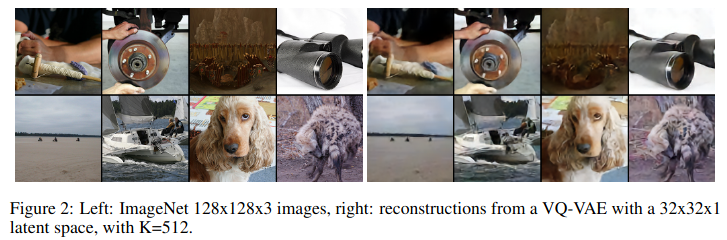
\includegraphics[width=1\textwidth]{images/D3.png}
    \label{fig:MHA2}
\end{figure}
The advantages are:
\begin{compactitemize}
    \item Learn domain-specific features, outperforming handcrafted codecs at low bitrates.
    \item Generates visually coherent reconstructions usin fewer bits.
\end{compactitemize}

\subsection{Learnable Prior in VQ-VAE}
A VQ-VAE learns three main components: an encoder, a decoder, and a codebook of discrete learnable embeddings.  
However, the model does not learn any distribution over the latent codes. This becomes a problem when we want to generate new images.

To synthesize new samples, we would ideally sample vectors from the codebook.  
But if we choose these codes randomly, the resulting images have no meaning: the decoder receives sequences of embeddings that do not correspond to any pattern that occurred in real data.

To fix this, the idea is to \textbf{learn the distribution of the discrete latent codes}.  
In practice:

\begin{compactitemize}
    \item we encode the training images using the VQ-VAE encoder to obtain sequences of codebook indices;
    \item we train a second generative model (e.g., PixelCNN or a Transformer) on these sequences;
    \item this model learns the true distribution over the discrete latent space;
    \item once trained, we can sample new sequences of latent codes from this learned prior;
    \item finally, we pass these sampled codes to the VQ-VAE decoder to generate meaningful new images.
\end{compactitemize}

In this way, the VQ-VAE becomes a complete generative model:  
it not only reconstructs existing inputs, but can also produce new coherent images because sampling occurs from a \textbf{learned prior} rather than from random codebook choices.
\begin{figure}[H]
    \centering
    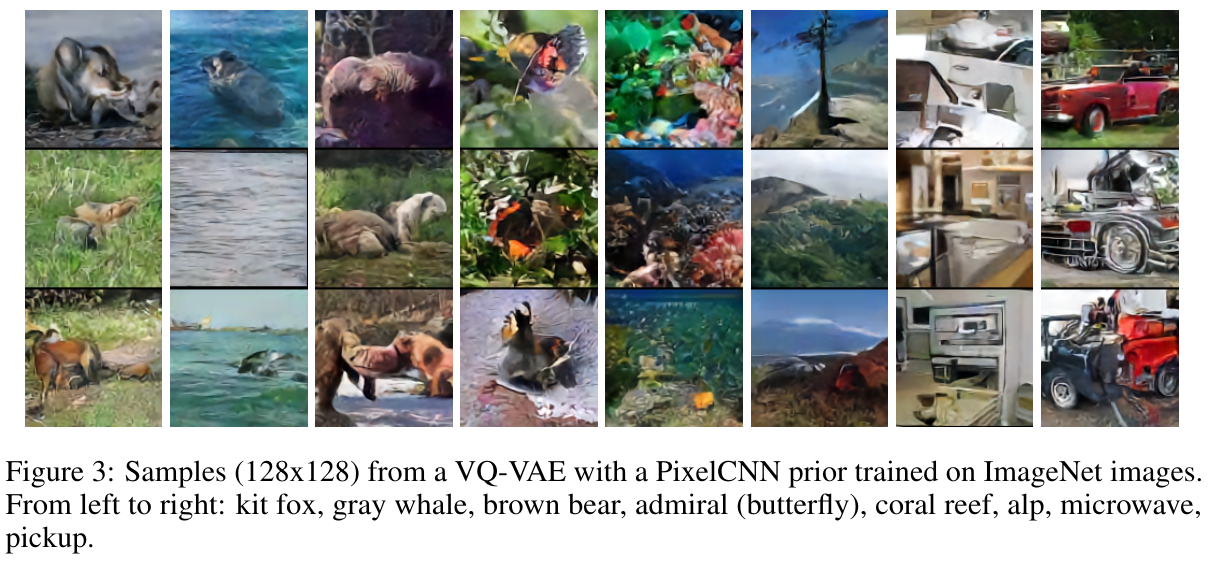
\includegraphics[width=1\textwidth]{images/D4.png}
    \label{fig:MHA2}
\end{figure}

\section{Autoregressive Models (PixelCNN)}
\begin{wrapfigure}{r}{0.3\textwidth}
    \centering
    \vspace{-10pt}
    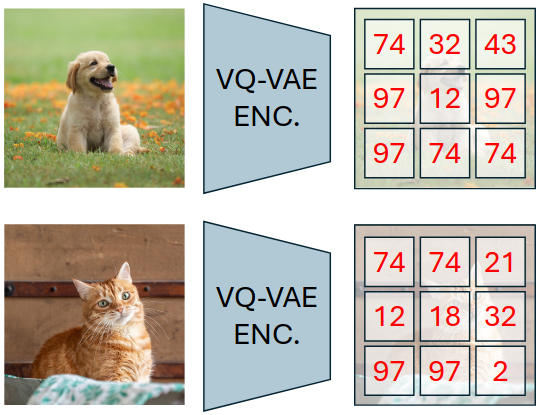
\includegraphics[width=\linewidth]{images/D5.png}
    \label{fig:Scaled Dot Product Attention}
    \vspace{-10pt}
\end{wrapfigure}
With the VQ-VAE model, we have a set of training examples expressed as sequences of \textbf{discrete symbols}:
\[
\{ \mathbf{z}^{(i)} = (z^{(i)}_{1}, z^{(i)}_{2}, \ldots, z^{(i)}_{T}) \}_{i=1}^{N}
\qquad \text{dove } z^{(i)}_{t} \in \{1, \ldots, K\}.
\]

The objective is to learn a generative model (learned prior) on top of these codes, which defines a parametric distribution over sequences of discrete latent variables:
\[
p_{\varepsilon_z}(z), \qquad z = (z_1, z_2, \ldots, z_T), \quad z_t \in \{1, \ldots, K\}.
\]

The main idea is to represent the joint density as a product of conditional distributions, using the chain rule of probability. In particular, the prior \(p_{\varepsilon_z}(z)\) can be learned through an autoregressive factorization of the joint density:
\[
p_{\varepsilon_z}(z) = \prod_{t=1}^{T} p_{\varepsilon_z}(z_t \mid z_{<t}),
\]
where each latent code \(z_t\) is predicted conditioned on all previous codes in the sequence.

To understand this factorization, we start from the definition of conditional probability:
\[
p(A \mid B) = \frac{p(A,B)}{p(B)} \qquad \Longleftrightarrow \qquad p(A,B) = p(A \mid B) \, p(B).
\]

By recursively applying this definition to a sequence of random variables \( z = (z_1, z_2, \ldots, z_T) \), the joint distribution can be decomposed as follows:
\begin{equation}
    \begin{split}
    p(z_1, z_2, \ldots, z_T) 
    &= p(z_T \mid z_1, \ldots, z_{T-1}) \, p(z_1, \ldots, z_{T-1}) \\
    &= p(z_T \mid z_{<T}) \, p(z_1, \ldots, z_{T-1}) \\
    &= p(z_T \mid z_{<T}) \, p(z_{T-1} \mid z_{<T-1}) \, p(z_1, \ldots, z_{T-2}) \\
    &= \cdots \\
    &= p(z_T \mid z_{<T}) \, p(z_{T-1} \mid z_{<T-1}) \, \cdots \, p(z_2 \mid z_1) \, p(z_1) \\
    &= \prod_{t=1}^{T} p(z_t \mid z_{<t}).
    \end{split}
\end{equation}

\begin{wrapfigure}{r}{0.4\textwidth}
    \centering
    \vspace{-10pt}
    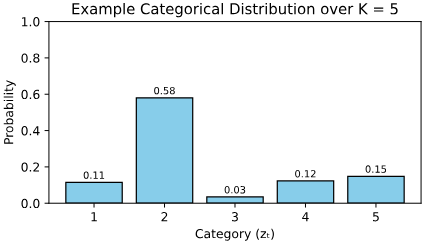
\includegraphics[width=\linewidth]{images/D6.png}
    \label{fig:Scaled Dot Product Attention}
    \vspace{-10pt}
\end{wrapfigure}
In this way, each latent variable is modeled conditioned on the previous ones, allowing the learning of an autoregressive sequential distribution over the discrete codes.

Each latent variable \(z_t\) is a discrete symbol taken from a codebook of size \(K\). In other words, the latent space is categorical, and each \(z_t\) can take one of \(K\) possible values:
\[
z_t \in \{1, \ldots, K\}.
\]

Accordingly, each conditional distribution in the autoregressive factorization can be modeled as a categorical distribution (also called a \emph{multinomial with one trial}):
\[
p_{\varepsilon_z}(z_t \mid z_{<t}) = \mathrm{Cat}(z_t; \pi_{\theta_z}(z_{<t})),
\]
where \(\pi_{\theta_z}(z_{<t})\) represents the vector of probabilities over the \(K\) codebook entries, conditioned on all previous latent variables \(z_{<t} = (z_1, \ldots, z_{t-1})\).  

In this way, the model learns a distribution over the discrete codes at each time step, taking into account the history of the sequence, which allows it to capture sequential dependencies in the latent space.


Each conditional distribution in the autoregressive factorization can be modeled as a categorical distribution:
\[
p_{\theta_z}(z_t \mid z_{<t}) = \mathrm{Cat}(z_t; \pi{\theta}(z_{<t})), \qquad z_t \in \{1, \ldots, K\},
\]
where \(\pi_{\theta}(z_{<t}) \in \mathbb{R}^{K \times 1}\) is the predicted probability vector over the \(K\) codebook entries. This vector can be parametrized by a neural network, which allows the model to flexibly learn how the probability of each code depends on the previous latent variables.  

Common choices for modeling \(p_{\theta_z}\) include:

\begin{compactitemize}
    \item \textbf{Pixel Recurrent Neural Networks (PixelRNN)}: uses recurrent connections over the sequence, less common for image latents.
    \item \textbf{PixelCNN}: a convolutional approach that is aware of the spatial grid structure, often used for image-based latents.
    \item \textbf{Transformer}: uses flexible attention-based mechanisms to model dependencies over the entire sequence, providing powerful context modeling.
\end{compactitemize}

In summary, by parameterizing each conditional as a neural network-predicted categorical distribution, the autoregressive model can capture complex sequential dependencies in the discrete latent space, allowing for rich generative modeling.

\subsection{PixelCNN: Inference}
The general idea is to model the prior over discrete latent variables 
\[
z \in \{1, \dots, K\}^{H \times W}
\] 
using a 2D autoregressive model. This is typically implemented via a (modified) Convolutional Neural Network (CNN), such as a PixelCNN.  

The joint distribution of the latents is factorized in raster scan order (row by row, left to right):
\[
p_{\theta_z}(z) = \prod_{i=1}^{H} \prod_{j=1}^{W} p_{\theta_Z}(z_{i,j} \mid z_{<i,j}),
\]
where \(z_{<i,j}\) denotes all previously generated pixels (or latent variables) in the raster scan order.  


Each conditional distribution 
\[
p_{\theta_z}(z_{i,j} \mid z_{<i,j})
\] 
is modeled as a categorical distribution whose probabilities are predicted by a convolutional neural network with \emph{masking} (\textbf{causal convolutions}), ensuring that no future pixel information is used when predicting the current pixel.

\[
p_{\theta_z}(z_{i,j} \mid z_{<i,j}) = \mathrm{Cat}(z_{i,j}; \pi_{\theta_z}(z_{<i,j})), 
\quad \pi_{\theta_z}(z_{<i,j}) = \mathrm{PixelCNN}(z_{<i,j}; \theta_z)
\]

\textbf{Inference (Sampling).}  
Sampling is performed sequentially following the raster scan order:

\begin{enumerate}
    \item Start with an empty image or latent grid.  
    \item For each pixel or latent variable \((i,j)\):
    \begin{enumerate}
        \item Perform a forward pass through the PixelCNN to obtain the conditional distribution \(\pi_{\theta_z}(z_{<i,j})\).  
        \item Sample \(z_{i,j}\) from the predicted categorical distribution:
        \[
        z_{i,j} \sim p_{\theta_z}(z_{i,j} \mid z_{<i,j}).
        \]  
        \item Fill in the grid sequentially, one pixel at a time.
    \end{enumerate}
\end{enumerate}

This approach allows the model to capture complex spatial dependencies among the latent variables, while maintaining a fully probabilistic generative model over the 2D latent grid.

\subsection{PixelCNN: Sampling}
At generation time, pixel are sampled one by one, in raster-scan order (left-to-right, top-to-bottom), using the predicted distribution conditioned on previous generated pixel.

This proccess is inherently \textbf{slow}, as each pixel depends on all previous one, but this ensueres valide sample frome the model.

This proccess lead at the fact that this infernce cannot be parallelized and the sampling time scales linearly with the number of pixel.

\subsection{Causal Convolutions}

In autoregressive models, such as PixelCNN, it is crucial to ensure that the prediction at position \((i,j)\) only depends on previously generated positions. This is necessary to avoid \textbf{information leakage}, i.e., the network accidentally using information from pixels it is supposed to predict.  

\begin{wrapfigure}{r}{0.14\textwidth}
    \centering
    \vspace{-10pt}
    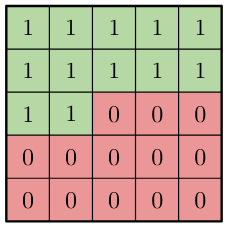
\includegraphics[width=\linewidth]{images/D7.png}
    \label{fig:Scaled Dot Product Attention}
    \vspace{-10pt}
\end{wrapfigure}
To enforce this constraint, PixelCNN uses \textbf{masked convolutions}. The basic idea is to prevent the convolutional kernel from “seeing” future pixels. This is typically implemented by \textbf{element-wise multiplying the convolutional kernel with a binary mask} before each forward pass. Such a mask is usually \textbf{hard-coded}, meaning that the positions that can be accessed are predefined and fixed, not learned by the network.  

\begin{infobox}[Hard-coded Binary Mask]
A \textbf{hard-coded binary mask} is a matrix of 0s and 1s that is multiplied element-wise with the convolutional kernel. 

- \textbf{1} indicates that the position is allowed to contribute to the output (can be “seen” by the convolution).  
- \textbf{0} indicates that the position is blocked (cannot be used).  

In a 2D autoregressive setting, this ensures that the convolution only attends to past pixels (above and to the left), enforcing the autoregressive constraint.
\end{infobox}

For 2D data such as images, PixelCNN typically uses two types of masks:

\begin{compactitemize}
    \item \textbf{Mask type A}: excludes the current pixel \((i,j)\). This is used in the \textbf{first layer} only, to enforce strict causality and prevent the network from seeing the pixel it is trying to predict.  
    \item \textbf{Mask type B}: includes the current pixel \((i,j)\). This is used in \textbf{all subsequent layers}, allowing the network to incorporate richer context from the feature maps of previous layers while still respecting the autoregressive property.  
\end{compactitemize}

\begin{infobox}[Why this distinction?]
- Type A is necessary in the \textbf{first layer} because at that stage the network has not yet seen any features derived from the current pixel, so strict causality must be enforced.  
- Type B is used in deeper layers because the original pixel at \((i,j)\) was never observed in the first layer, so allowing access to this position in the feature maps does not violate the autoregressive property. Instead, it provides \textbf{richer context} to the network, improving its ability to model complex dependencies.
\end{infobox}

\subsection{PixelCNN: Training}
During training, \textbf{PixelCNN suffers from slow sampling}, since its autoregressive structure requires the model to generate each pixel sequentially. For every pixel location, the model must perform a forward pass conditioned on all previously generated pixels. This strict dependency makes sampling extremely slow, especially for high-resolution images.

To address this issue, we use \textbf{Teacher Forcing}, which becomes feasible during training because \textbf{ground-truth pixel values (or latent codes) are available}. Instead of allowing the model to generate one pixel at a time and feeding its own predictions back as inputs, Teacher Forcing provides the true pixel values at each location as conditioning information. As a result, \textbf{the model does not rely on its own predictions during training}, eliminating the need for sequential generation.
\begin{wrapfigure}{r}{0.6\textwidth}
    \centering
    \vspace{-10pt}
    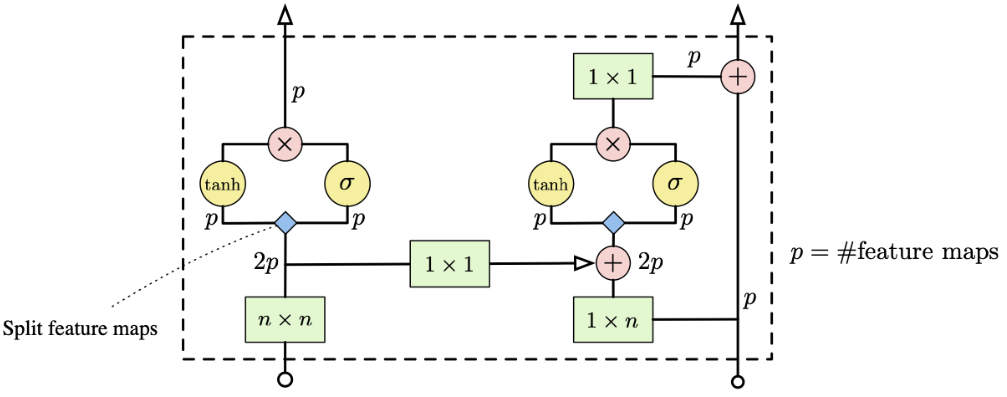
\includegraphics[width=\linewidth]{images/D9.png}
    \label{fig:Scaled Dot Product Attention}
    \vspace{-10pt}
\end{wrapfigure}
With Teacher Forcing, \textbf{PixelCNN can predict all pixels in parallel through a single forward pass}, since each prediction is conditioned on the ground-truth values rather than sampled outputs. This makes training highly efficient: \textbf{no autoregressive sampling loop is required}, and the entire image can be processed simultaneously. Consequently, even though PixelCNN still requires sequential sampling during inference, \textbf{training becomes fully parallelizable and drastically faster}, enabling practical optimization of autoregressive models despite slow sampling at inference time.
\begin{figure}[H]
    \centering
    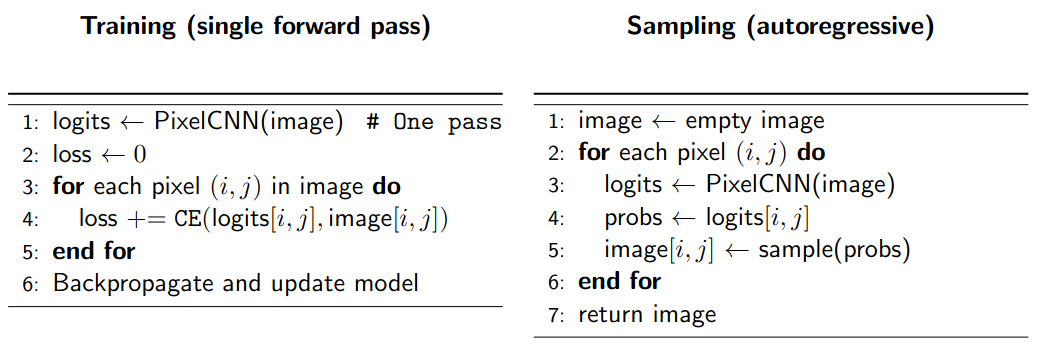
\includegraphics[width=1\textwidth]{images/D8.png}
    \label{fig:MHA2}
\end{figure}

\subsection{PixelCNN: Likelyhood and Anomaly Detection}
PixelCNN models the exact data likelihood using an autoregressive factorization of the image distribution:

\[
\log p(x) = \sum_{i,j} \log p(x_{i,j} \mid x_{<i,j})
\]

This likelihood can be computed efficiently in a single forward pass by using masked convolutions, which ensure that each pixel prediction depends only on the valid preceding pixels. As a result, PixelCNN allows us to assign a probability score (or log-likelihood) to any image directly.

This capability enables several important applications. One key use case is \textbf{anomaly detection}, where unusual or corrupted images typically exhibit very low likelihood under the model. Another closely related application is \textbf{novelty detection}, in which out-of-distribution (OOD) samples can be identified by thresholding their likelihood scores. High-likelihood images are considered consistent with the training distribution, while low-likelihood ones are flagged as novel or anomalous.

\subsection{Summary}
\textbf{VQ-VAE: Vector Quantized Variational Autoencoder:} 
Learns a \textbf{discrete latent space} through vector quantization. The encoder maps inputs to discrete latent codes using a learned codebook, while the decoder reconstructs the original input from these codes. This framework enables \textbf{efficient and compressible representations} by replacing continuous latent variables with discrete embeddings.

\textbf{PixelCNN:} 
PixelCNN models the \textbf{joint distribution over the discrete latent codes} produced by the VQ-VAE encoder. It is trained directly on these latents to learn a powerful generative prior. Once trained, PixelCNN can sample new latent code grids, which are then passed to the VQ-VAE decoder to generate images.

\textbf{Combined Pipeline:} 
The overall system works in two stages:  
\begin{compactitemize}
    \item \textbf{Train the VQ-VAE} to learn a discrete latent representation and a decoder capable of reconstructing images from latent codes.
    \item \textbf{Train PixelCNN on the discrete latent maps} to model their distribution and serve as a generative prior.    
\end{compactitemize}

At generation time, samples are drawn from the PixelCNN prior and subsequently decoded using the VQ-VAE decoder, producing fully generated images.

\section{Gumbel-Softmax}
\begin{wrapfigure}{r}{0.3\textwidth}
    \centering
    \vspace{-10pt}
    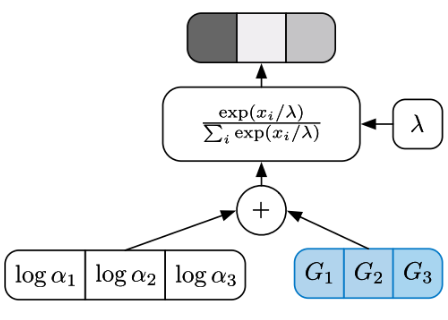
\includegraphics[width=\linewidth]{images/D10.png}
    \label{fig:Scaled Dot Product Attention}
    \vspace{-10pt}
\end{wrapfigure}
As we saw in the first example of this chapter, the \textbf{argmax} function is not differentiable and therefore breaks the training process. We also discussed a workaround known as the \textbf{Straight-Through Estimator (STE)}, which consists of performing the discrete sampling during the forward pass while treating the operation as the identity function during the backward pass in order to propagate gradients.

However, there exists another approach to avoid the non-differentiability of the argmax: the \textbf{Gumbel-Softmax} trick. This method allows us to sample from a categorical distribution during the forward pass of a neural network while still maintaining differentiability with respect to the logits.

In this setting, the encoder produces logits over the codebook entries. Instead of selecting a single discrete index, we sample a \emph{soft} categorical vector using the Gumbel-Softmax formulation:

\[
y_k = \frac{\exp\left( \frac{\log \pi_k + g_k}{\lambda} \right)}
{\sum_{j} \exp\left( \frac{\log \pi_j + g_j}{\lambda} \right)}
\]

where:
\begin{compactitemize}
    \item $\pi_k$ are the unnormalized probabilities (logits) of the categorical distribution,
    \item $g_k$ are i.i.d.\ Gumbel noise samples,
    \item $\lambda$ is the temperature parameter controlling the softness of the distribution.
\end{compactitemize}

As $\lambda \to 0$, the distribution becomes increasingly sharp and approximates a one-hot categorical sample. For higher values of $\lambda$, the output is smoother and fully differentiable. This mechanism shares strong similarities with the \textbf{Reparameterization Trick} used in continuous VAEs, as it enables gradient-based optimization through a stochastic sampling step. The Gumbel-Softmax therefore provides a principled and differentiable alternative to the STE for learning discrete latent representations.
\begin{figure}[H]
    \centering
    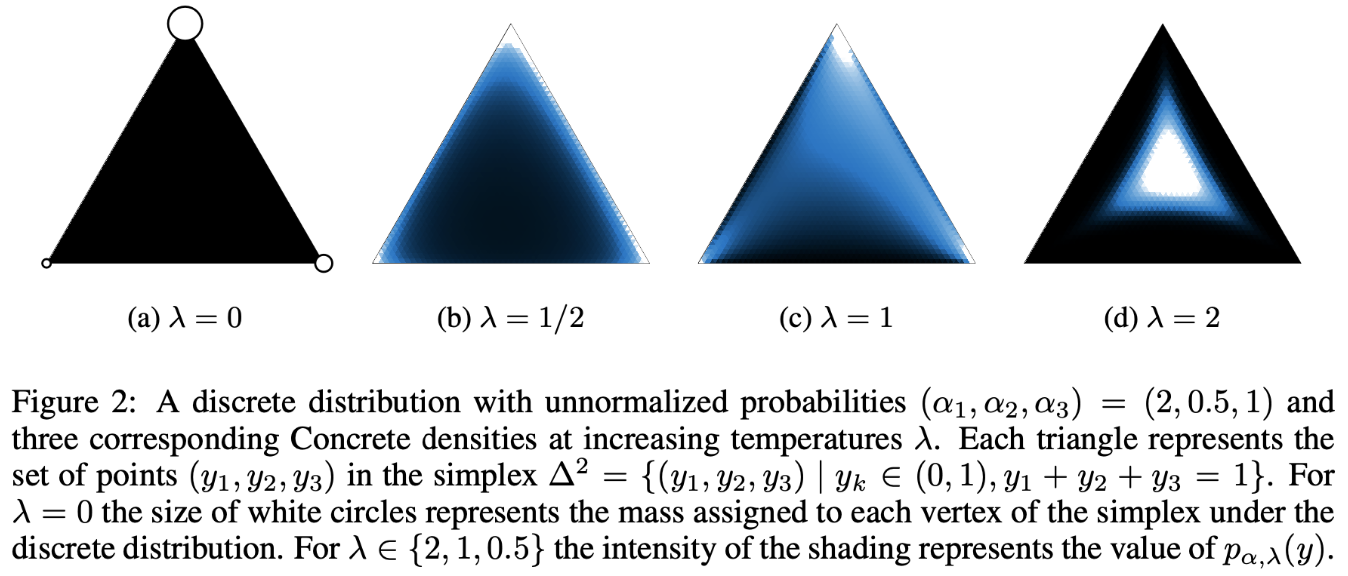
\includegraphics[width=1\textwidth]{images/D11.png}
    \label{fig:MHA2}
\end{figure}

\begin{figure}[H]
    \centering
    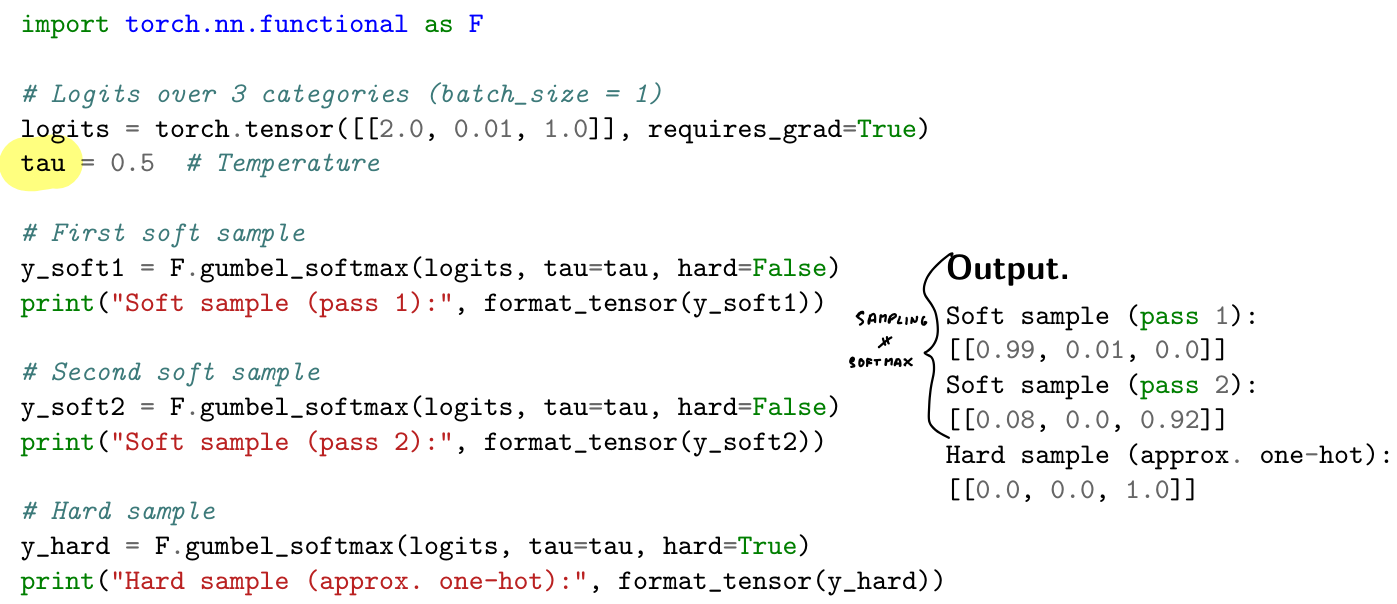
\includegraphics[width=1\textwidth]{images/D12.png}
    \label{fig:MHA2}
\end{figure}
\begin{infobox}[Sampling vs Softmax]
    When using the standard \textbf{softmax} function on the logits produced by the encoder, the output is \emph{deterministic}.  
    Given the same input $x$, the encoder always produces the same logits, and the softmax always produces the same probability vector.  
    This is useful for classification, but it does \emph{not} allow us to sample discrete latent variables.

    In contrast, the \textbf{Gumbel-Softmax} introduces \emph{stochasticity} by adding Gumbel noise to the logits before applying a temperature-controlled softmax.  
    This means that even if the encoder outputs the same logits at every forward pass, the addition of random Gumbel noise causes the resulting Gumbel-Softmax vector to be \textbf{different each time}.  
    Thus, the model can produce \emph{different samples} from the same categorical distribution.

    This is the key advantage:  
    \begin{compactitemize}
        \item We want to \textbf{sample} a discrete latent variable (like choosing a codebook entry).  
        \item But we also want the entire operation to remain \textbf{differentiable}, so gradients can pass through the sampling step.
    \end{compactitemize}

    The Gumbel-Softmax bridges this gap:
    \begin{compactitemize}
        \item It behaves like sampling because the Gumbel noise randomizes the output.  
        \item It remains differentiable because the output after applying the temperature softmax is still a continuous vector.
    \end{compactitemize}
\end{infobox}
\begin{figure}[H]
    \centering
    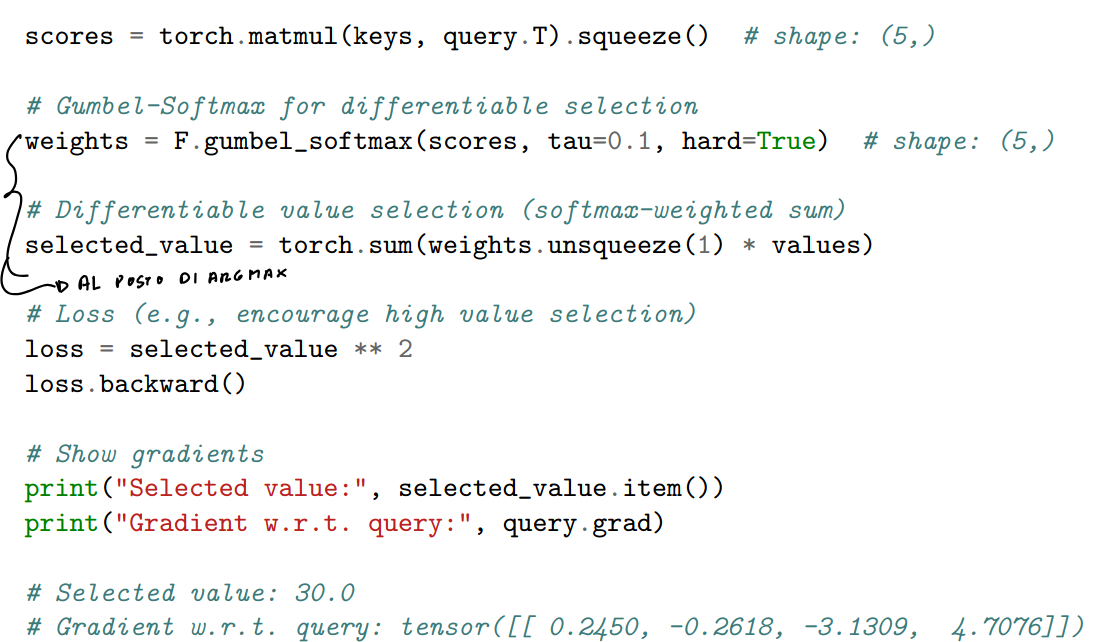
\includegraphics[width=1\textwidth]{images/D13.png}
    \caption{The initial example: Now}
    \label{fig:MHA2}
\end{figure}